\documentclass[a4paper]{article}
\usepackage[a4paper, margin=1in]{geometry}
% Some basic packages
\usepackage[utf8]{inputenc}
\usepackage[T1]{fontenc}
\usepackage{textcomp}
\usepackage[dutch]{babel}
\usepackage{url}
\usepackage{graphicx}
\usepackage{float}
\usepackage{booktabs}
\usepackage{enumitem}

\pdfminorversion=7

% Don't indent paragraphs, leave some space between them
\usepackage{parskip}

% Hide page number when page is empty
\usepackage{emptypage}
\usepackage{subcaption}
\usepackage{multicol}
\usepackage{xcolor}

% Other font I sometimes use.
% \usepackage{cmbright}

% Math stuff
\usepackage{amsmath, amsfonts, mathtools, amsthm, amssymb}
% Fancy script capitals
\usepackage{mathrsfs}
\usepackage{cancel}
% Bold math
\usepackage{bm}
% Some shortcuts
\newcommand\N{\ensuremath{\mathbb{N}}}
\newcommand\R{\ensuremath{\mathbb{R}}}
\newcommand\Z{\ensuremath{\mathbb{Z}}}
\renewcommand\O{\ensuremath{\emptyset}}
\newcommand\Q{\ensuremath{\mathbb{Q}}}
\newcommand\C{\ensuremath{\mathbb{C}}}

% Easily typeset systems of equations (French package)
\usepackage{systeme}

% Put x \to \infty below \lim
\let\svlim\lim\def\lim{\svlim\limits}

%Make implies and impliedby shorter
\let\implies\Rightarrow
\let\impliedby\Leftarrow
\let\iff\Leftrightarrow
\let\epsilon\varepsilon

% Add \contra symbol to denote contradiction
\usepackage{stmaryrd} % for \lightning
\newcommand\contra{\scalebox{1.5}{$\lightning$}}

% \let\phi\varphi

% Command for short corrections
% Usage: 1+1=\correct{3}{2}

\definecolor{correct}{HTML}{009900}
\newcommand\correct[2]{\ensuremath{\:}{\color{red}{#1}}\ensuremath{\to }{\color{correct}{#2}}\ensuremath{\:}}
\newcommand\green[1]{{\color{correct}{#1}}}

% horizontal rule
\newcommand\hr{
    \noindent\rule[0.5ex]{\linewidth}{0.5pt}
}

% hide parts
\newcommand\hide[1]{}

% si unitx
\usepackage{siunitx}
\sisetup{locale = FR}

% Environments
\makeatother
% For box around Definition, Theorem, \ldots
\usepackage{mdframed}
\mdfsetup{skipabove=1em,skipbelow=0em}
\theoremstyle{definition}
\newmdtheoremenv[nobreak=true]{definitie}{Definitie}
\newmdtheoremenv[nobreak=true]{eigenschap}{Eigenschap}
\newmdtheoremenv[nobreak=true]{gevolg}{Gevolg}
\newmdtheoremenv[nobreak=true]{lemma}{Lemma}
\newmdtheoremenv[nobreak=true]{propositie}{Propositie}
\newmdtheoremenv[nobreak=true]{stelling}{Stelling}
\newmdtheoremenv[nobreak=true]{wet}{Wet}
\newmdtheoremenv[nobreak=true]{postulaat}{Postulaat}
\newmdtheoremenv{conclusie}{Conclusie}
\newmdtheoremenv{toemaatje}{Toemaatje}
\newmdtheoremenv{vermoeden}{Vermoeden}
\newtheorem*{herhaling}{Herhaling}
\newtheorem*{intermezzo}{Intermezzo}
\newtheorem*{notatie}{Notatie}
\newtheorem*{observatie}{Observatie}
\newtheorem*{oef}{Oefening}
\newtheorem*{opmerking}{Opmerking}
\newtheorem*{praktisch}{Praktisch}
\newtheorem*{probleem}{Probleem}
\newtheorem*{terminologie}{Terminologie}
\newtheorem*{toepassing}{Toepassing}
\newtheorem*{uovt}{UOVT}
\newtheorem*{vb}{Voorbeeld}
\newtheorem*{vraag}{Vraag}

\newmdtheoremenv[nobreak=true]{definition}{Definition}
\newtheorem*{eg}{Example}
\newtheorem*{notation}{Notation}
\newtheorem*{previouslyseen}{As previously seen}
\newtheorem*{remark}{Remark}
\newtheorem*{note}{Note}
\newtheorem*{problem}{Problem}
\newtheorem*{observe}{Observe}
\newtheorem*{property}{Property}
\newtheorem*{intuition}{Intuition}
\newmdtheoremenv[nobreak=true]{prop}{Proposition}
\newmdtheoremenv[nobreak=true]{theorem}{Theorem}
\newmdtheoremenv[nobreak=true]{corollary}{Corollary}

% End example and intermezzo environments with a small diamond (just like proof
% environments end with a small square)
\usepackage{etoolbox}
\AtEndEnvironment{vb}{\null\hfill$\diamond$}%
\AtEndEnvironment{intermezzo}{\null\hfill$\diamond$}%
% \AtEndEnvironment{opmerking}{\null\hfill$\diamond$}%

% Fix some spacing
% http://tex.stackexchange.com/questions/22119/how-can-i-change-the-spacing-before-theorems-with-amsthm
\makeatletter
\def\thm@space@setup{%
  \thm@preskip=\parskip \thm@postskip=0pt
}


% Exercise 
% Usage:
% \oefening{5}
% \suboefening{1}
% \suboefening{2}
% \suboefening{3}
% gives
% Oefening 5
%   Oefening 5.1
%   Oefening 5.2
%   Oefening 5.3
\newcommand{\oefening}[1]{%
    \def\@oefening{#1}%
    \subsection*{Oefening #1}
}

\newcommand{\suboefening}[1]{%
    \subsubsection*{Oefening \@oefening.#1}
}


% \lecture starts a new lecture (les in dutch)
%
% Usage:
% \lecture{1}{di 12 feb 2019 16:00}{Inleiding}
%
% This adds a section heading with the number / title of the lecture and a
% margin paragraph with the date.

% I use \dateparts here to hide the year (2019). This way, I can easily parse
% the date of each lecture unambiguously while still having a human-friendly
% short format printed to the pdf.

\usepackage{xifthen}
\def\testdateparts#1{\dateparts#1\relax}
\def\dateparts#1 #2 #3 #4 #5\relax{
    \marginpar{\small\textsf{\mbox{#1 #2 #3 #5}}}
}

\def\@lecture{}%
\newcommand{\lecture}[3]{
    \ifthenelse{\isempty{#3}}{%
        \def\@lecture{Lecture #1}%
    }{%
        \def\@lecture{Lecture #1: #3}%
    }%
    \subsection*{\@lecture}
    \marginpar{\small\textsf{\mbox{#2}}}
}



% These are the fancy headers
\usepackage{fancyhdr}
\pagestyle{fancy}

% LE: left even
% RO: right odd
% CE, CO: center even, center odd
% My name for when I print my lecture notes to use for an open book exam.
% \fancyhead[LE,RO]{Gilles Castel}

\fancyhead[RO,LE]{\@lecture} % Right odd,  Left even
\fancyhead[RE,LO]{}          % Right even, Left odd

\fancyfoot[RO,LE]{\thepage}  % Right odd,  Left even
\fancyfoot[RE,LO]{}          % Right even, Left odd
\fancyfoot[C]{\leftmark}     % Center

\makeatother




% Todonotes and inline notes in fancy boxes
\usepackage{todonotes}
\usepackage{tcolorbox}

% Make boxes breakable
\tcbuselibrary{breakable}

% Verbetering is correction in Dutch
% Usage: 
% \begin{verbetering}
%     Lorem ipsum dolor sit amet, consetetur sadipscing elitr, sed diam nonumy eirmod
%     tempor invidunt ut labore et dolore magna aliquyam erat, sed diam voluptua. At
%     vero eos et accusam et justo duo dolores et ea rebum. Stet clita kasd gubergren,
%     no sea takimata sanctus est Lorem ipsum dolor sit amet.
% \end{verbetering}
\newenvironment{verbetering}{\begin{tcolorbox}[
    arc=0mm,
    colback=white,
    colframe=green!60!black,
    title=Opmerking,
    fonttitle=\sffamily,
    breakable
]}{\end{tcolorbox}}

% Noot is note in Dutch. Same as 'verbetering' but color of box is different
\newenvironment{noot}[1]{\begin{tcolorbox}[
    arc=0mm,
    colback=white,
    colframe=white!60!black,
    title=#1,
    fonttitle=\sffamily,
    breakable
]}{\end{tcolorbox}}




% Figure support as explained in my blog post.
\usepackage{import}
\usepackage{xifthen}
\usepackage{pdfpages}
\usepackage{transparent}
\newcommand{\incfig}[1]{%
    \def\svgwidth{\columnwidth}
    \import{./figures/}{#1.pdf_tex}
}

% Fix some stuff
% %http://tex.stackexchange.com/questions/76273/multiple-pdfs-with-page-group-included-in-a-single-page-warning
\pdfsuppresswarningpagegroup=1

\title{\Huge{Hw 8}}
\author{\huge{Daniel Yu}}
\date{November 6, 2024}

\pdfsuppresswarningpagegroup=1

\begin{document}
\maketitle
\newpage% or \cleardoublepage
% \pdfbookmark[<level>]{<title>}{<dest>}
\pagebreak
\begin{enumerate}
  \item Let $X_n$ be an irreducible, aperiodic finite-state Markov chain with transition matrix $P =
    (p_{i,j})_{i,j}$, and a stationary distribution $\pi = (\pi_1, \pi_2, \ldots, \pi_n)$. Let $Y_n$ keep track of the two previous states — that is, $Y_n = (X_{n - 1}, X_n)$. Show that $Y_n$ is a Markov chain, and compute its stationary distribution (in terms of P and $\pi$). 
 
    \noindent\hrulefill

    \begin{proof}
      Since $X_n, X_{n - 1}$ are previous states in the Markov Chain, then they will follow the transition matrix $P$ and have the same markov chain dynamics.

      Notice that $Y_n$ is a markov chain because $P[Y_{n} \mid Y_{n-1}, Y_{n-2}, \ldots, Y_{1}] = P[Y_{n} \mid Y_{n-1}]$ because:
      \begin{align*}
        P[Y_n \mid Y_{n-1}, Y_{n-2}, \ldots, Y_{1}] &= P[(X_{n-1}, X_n) \mid (X_{n-2}, X_{n-1}), (X_{n-3}, X_{n-2}) \ldots, (X_{2}, X_{1})] \\
                                                    &= P[(X_{n-1}, X_{n}) \mid (X_{n-2}, X_{n-1})] \\
                                                    &= P[Y_n \mid Y_{n-1}] 
                                                  .\end{align*}
    Now consider, the distribution of $Y_n$.
      \begin{align*}
        P(Y_{n} = (c,d) \mid Y_{n-1} =(a,b)) &= P[(X_{n-1}, X_{n}) = (c,d) \mid (X_{n-2}, X_{n-1}) = (a,b)  ]\\ 
                                                                    &=  P[(X_{n-1}, X_{n}) = (c,d) \mid (X_{n-2},X_{n-1}) = (a,b), X_{n-1} = X_{n-1}] + \\
                                                                    &P[(X_{n-1}, X_{n}) = (c,d) \mid (X_{n-2},X_{n-1}) = (a,b), X_{n-1} \neq X_{n-1}] \\
                                                                    &= P[(X_{n-1}, X_{n}) = (b,d) \mid (X_{n-2},X_{n-1}) = (a,b), X_{n-1} = X_{n-1}] + 0\\
                                                                    &= P[X_{n} = d \cap X_{n-1} = b \cap X_{n-2}=a] \\
                                                                    &= P[X_{n} = d \mid X_{n-1} = b \cap X_{n-2} = a] \cdot P[X_{n-1} = b \mid X_{n-2} = a] \cdot P[X_{n-2} = a] \\
                                                                    &= P[X_n =d \mid X_{n-1} =b] \cdot P[X_{n-1} =b \mid X_{n-2}=a] \cdot P[X_{n-2}=a] \\
                                                                    &= P[X_n =d \mid X_{n-1} =b] \cdot P[X_{n-1} =b \mid X_{n-2}=a] \left( \sum_{i \in \Omega} P[X_{n-2} = a \mid X_0 = i] \right) \\ 
                                                                    &= P_{b,d} P_{a,b} \left( v \cdot P^{n-2} \right)_{a}  \\
                                                                    &\text{ as $n \to \infty$}\\
                                                                    &= P_{b,d} P_{a,b} \pi_{a}  
                                                                  .\end{align*}
    The probability matrix $P_{Y_n} ((b,c),(a,b)) = P_{b,c} P_{a,b}$ and the stationary distribution is $\pi = P_{b,d} P_{a,b} \pi_{a}$.
  \end{proof}
  \item Let us consider a very simple version of monopoly: there are 4 squares, one marked ‘GO,’ the
next ’Baltic’, the third ’Free Parking’, and the fourth ’Boardwalk,’ arranged in a circle. At any
turn, we toss two fair coins; we advance 1 square if both are tails, 2 if exactly one is heads, and
3 if both are heads. If we start at ’GO’, what is the expected time when we first return to ’GO’ ?
What is the expected number of visits to ’Boardwalk’ before the first return to ’GO’ ?

\noindent\hrulefill

\begin{proof}
  The transition matrix would be 
  \[
  P = \begin{pmatrix} 
    0 & \frac{1}{4} & \frac{1}{2} & \frac{1}{4} \\
    \frac{1}{4} & 0 & \frac{1}{4} & \frac{1}{2} \\ 
    \frac{1}{2} & \frac{1}{4} & 0 & \frac{1}{4} \\
    \frac{1}{4} & \frac{1}{2} & \frac{1}{4} & 0 
  \end{pmatrix} 
  .\] 
  The markov chain would be of the form below.

\begin{figure}[H]
  \centering
  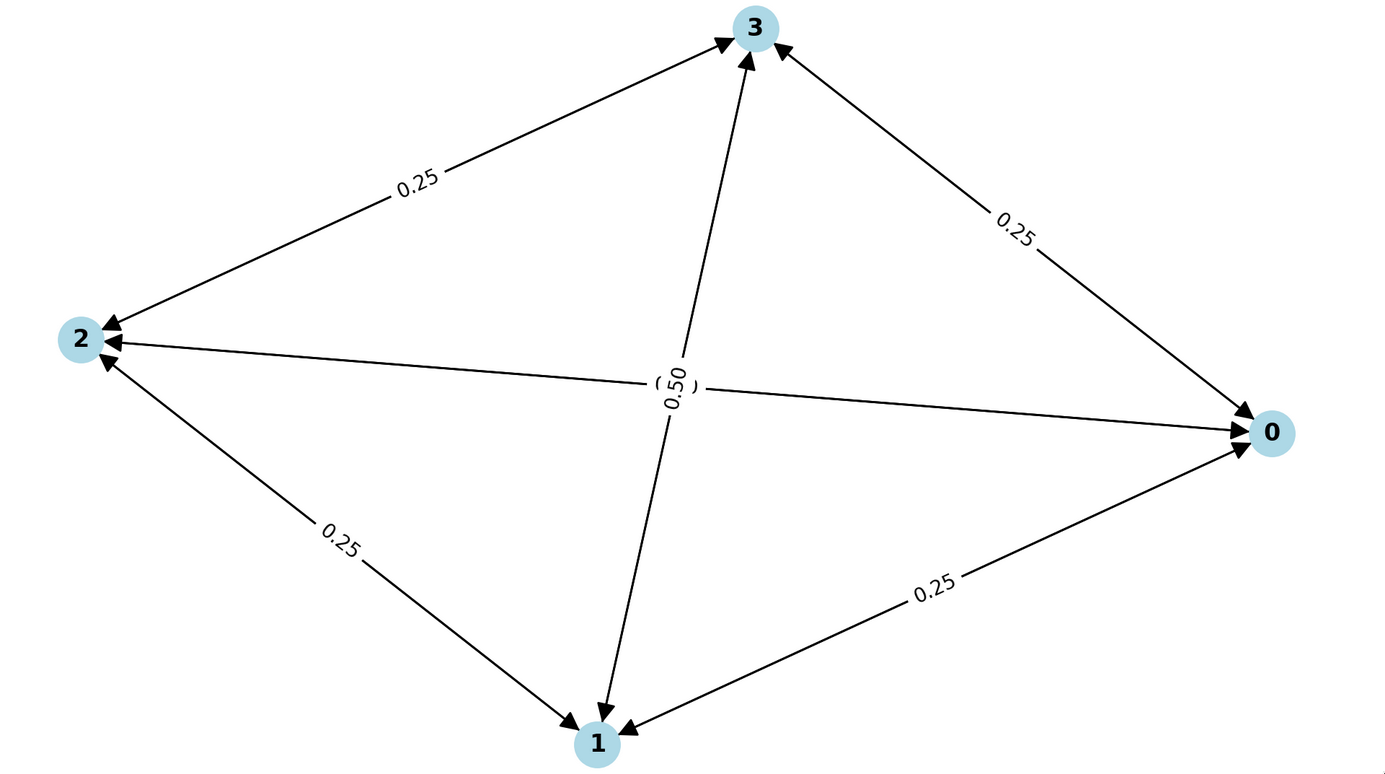
\includegraphics[width=0.8\textwidth]{assets/hw8_problem2.png}
  \caption{Markov Chain}
  \label{fig:hw8_problem2}
\end{figure}
Notice that $E[\text{ GO} \mid  \text{GO}]$ is just the sojurn time: $E[S_{\text{GO}} \mid X_0 = \text{GO}] = \frac{1}{\pi_{\text{GO}}}$. \\

Since $P$ is doubly stochastic, then $\pi$ is a constant vector, and $\pi = \begin{pmatrix} \frac{1}{4}\\ \frac{1}{4}\\ \frac{1}{4} \\ \frac{1}{4} \end{pmatrix}$. Thus, 
 \[
E[S_{\text{GO}} \mid X_0 = \text{GO}] = \frac{1}{.25} = 4 
.\] 


\end{proof}
\end{enumerate}
\end{document}
